\chapter{Návrh}
\label{ch:design}
Dalším krokem vývoje software je návrh, který pomůže získat celkovou představu o~aplikaci, jejích částech a případně problémových místech. V~rámci této kapitoly se budeme zabývat požadavky na aplikaci a tvorbou specifikace, které se následně vývojář bude držet. Součástí specifikace jsou~\hyperref[sc:user_roles]{uživatelské role},~\hyperref[sc:use_cases]{případy užití} a~\hyperref[sc:wireframes]{wireframy}, které vývojáři pomůžou získat představu o~grafické reprezentaci aplikace.

\section{Funkční požadavky}
\label{sc:functional_req}

\begin{requirment}{FP01 Metronom}{FP01}
    Aplikace zobrazí uživateli metronom. Uživatel má možnost zapnout či vypnout metronom a zvolit si rychlost.
\end{requirment}

\begin{requirment}{FP02 Akordy}{FP02}
    Aplikace umožní uživateli si zobrazit libovolnou podmnožinu akordů.
\end{requirment}

\begin{requirment}{FP03 Strumming pattern}{FP03}
    Aplikace zobrazí uživateli strumming pattern a metronom. Uživatel může ovládat metronom dle \hyperref[FP01]{FP01} a zobrazení strumming patternu reaguje na nastavení rychlosti metronomu.
\end{requirment}

\begin{requirment}{FP04 Vyhledávání}{FP04}
    Aplikace umožní uživateli vyhledávat písně, akordy a strumming patterny.
\end{requirment}

\begin{requirment}{FP05 Přechytávání akordů}{FP05}
    Aplikace umožní uživateli si vytvořit vlastní seznam akordů s volbou nastavení metronomu dle \hyperref[FP01]{FP01} a akordů dle \hyperref[FP02]{FP02}.
    Přihlášený uživatel má možnost si dané nastavení uložit pod libovolným jménem.
\end{requirment}

\begin{requirment}{FP06 Přechytávání akordů dle písně}{FP06}
    Aplikace zobrazí uživateli přechytávání akordů dle \hyperref[FP05]{FP05} s přednastavenými parametry podle vybrané písně.
\end{requirment}

\begin{requirment}{FP07 Zobrazení písně}{FP07}
    Aplikace zobrazí uživateli text písně, akordy písně a strumming pattern dle \hyperref[FP03]{FP03}. Uživatel má možnost přechodu na přechytávání akordů dle \hyperref[FP06]{FP06} a případně odkaz na přehrání písně na serveru třetí strany (např. youtube, spotify).
\end{requirment}

\begin{requirment}{FP08 Registrace}{FP08}
    Aplikace umožní zaregistrovat nového uživatele.
\end{requirment}

\begin{requirment}{FP09 Přihlášení}{FP09}
    Aplikace umožní uživateli se přihlásit.
\end{requirment}

\begin{requirment}{FP22 Odhlášení}{FP22}
    Aplikace umožní odhlásit přihlášeného uživatele.
\end{requirment}

\begin{requirment}{FP23 Úprava profilu}{FP23}
    Aplikace umožní přihlášenému uživateli měnit svoje údaje.
\end{requirment}

% \noindent \begin{minipage}{\textwidth}
%     \paragraph{FP13 Nastavení ladění} \label{FP13}
%     \begin{smallindent}{}
%         Aplikace nastaví ladění ukulele přihlášeného uživatele podle vstupu od uživatele.
%     \end{smallindent}
% \end{minipage}

\begin{requirment}{FP24 Označení písně jako oblíbená}{FP24}
    Aplikace umožní příhlášenému uživateli označit píseň jako oblíbenou.
\end{requirment}

\begin{requirment}{FP41 Vytvoření písně}{FP41}
    Aplikace umožňuje moderátorovi vytvořit nový záznam o písni.
\end{requirment}

\begin{requirment}{FP42 Úprava písně}{FP42}
    Aplikace umožňuje moderátorovi upravit existující záznam o písni.
\end{requirment}

\begin{requirment}{FP61 Úprava rolí uživatele}{FP61}
    Aplikace umožňuje administrátorovi změnit role uživatele.
\end{requirment}


\section{Nefunkční požadavky}
\label{sc:non_func_req}

\begin{requirment}{NP01 Kompatibilita}{NP01}
    Aplikace je dostupná přes webové rozhraní. Webové rozhraní poskytuje podporu pro prohlížeče Mozilla Firefox od verze 68, Google Chrome od verze 79 a Safari od verze 12.
\end{requirment}

\begin{requirment}{NP02 Podpora menších obrazovek}{NP02}
    Aplikace je responzivní, tedy se adaptuje na velikost obrazovky uživatele a podporuje dané prohlížeče na mobilních telefonech.
\end{requirment}

\begin{requirment}{NP03 SEO}{NP03}
    Aplikace je SEO-friendly, tedy splňuje všechny náležitosti pro internetové vyhledávače jako jsou Google nebo Seznam. Tyto náležitosti jsou testovány pomocí nástroje Google Lighthouse \cite{googlellc_2019_lighthouse}, kde aplikace musí dosáhnout celkového bodového ohodnocení alespoň 90 ze 100.
\end{requirment}

\begin{requirment}{NP04 API}{NP04}
    Aplikace vystavuje soukromé API a to ve formátu GraphQL.
\end{requirment}

\begin{requirment}{NP05 Rozšiřitelnost}{NP05}
    Aplikace je díky správnému návrhu a plánování možností rozšíření lehce rozšiřitelná.
\end{requirment}

\begin{requirment}{NP06 Lokalizace}{NP06}
    Aplikace je dostupná v anglickém jazyce.
\end{requirment}



\section{Uživatelské role}
\label{sc:user_roles}

\noindent \begin{minipage}{\textwidth}
    \paragraph{Uživatel}
    \begin{smallindent}{}
        Běžný uživatel, který se chce naučit hrát na ukulele nebo využít jinou funkcionalitu aplikace. Může použít metronom, učit se akordy, jejich přechytávání a nebo celou písničku.
        Má možnost se registrovat.
    \end{smallindent}
\end{minipage}


\noindent \begin{minipage}{\textwidth}
    \paragraph{Přihlášený uživatel}
    \begin{smallindent}{}
        To samé jako uživatel s možností se přihlásit, ukládat oblíbené písničky, vlastní přechytávání akordů. Dále má možnost si nastavit ladění vlastního ukulele, na což aplikace reaguje tak, že všude kde budou zobrazeny akordy, jmenovitě FP-002, FP-004-1, FP-004-2, tak má možnost přepnout mezi vlastním nastavením a výchozím.
    \end{smallindent}
\end{minipage}

\noindent \begin{minipage}{\textwidth}
    \paragraph{Moderátor}
    \begin{smallindent}{}
        To samé jako přihlášený uživatel s možností editovat písničky (akordy, strumming pattern, odkaz na ukázku).
    \end{smallindent}
\end{minipage}

\noindent \begin{minipage}{\textwidth}
    \paragraph{Administrátor}
    \begin{smallindent}{}
        To samé jako moderátor s možností upravovat role uživatelů.
    \end{smallindent}
\end{minipage}

\newpage
\section{Případy užití}
\label{sc:use_cases}

\begin{usecase}{PU01 Metronom}{uc01}
    Případ užití umožňuje uživateli nastavovat parametry metronomu a ovládat ho. Mezi parametry patří tempo a způsob ukazování tempa (zvuková signalizace, blikání, odpočet, nebo vybrace na telefonu).

    \begin{scenario}{HS: Zobrazení metronomu}{uc01:hs}
        \item Scénář začne když uživatel zobrazí tuto komponentu.
        \item Aplikace zobrazí metronom a k~němu příslušející nastavení
    \end{scenario}

    \begin{scenario}{AS01: Zapnutí metronomu}{uc01:as01}
        \item Scénař začne když uživatel klikne na tlačítko \enquote{Start}
        \item Aplikace spustí metronom s~nastavenými parametry.
        \begin{itemize}
            \item Aplikace reaguje na změny parametrů okamžitě.
        \end{itemize}
        \item Tlačítko \enquote{Start} se změní na tlačítko \enquote{Stop} a scénář končí.
    \end{scenario}

    \begin{scenario}{AS02: Vypnutí metronomu}{uc01:as02}
        \item Scénař začne když uživatel klikne na tlačítko \enquote{Stop}
        \item Aplikace vypne metronom.
        \item Tlačítko \enquote{Stop} se změní na tlačítko \enquote{Start} a scénář končí.
    \end{scenario}
\end{usecase}

\begin{usecase}{PU02 Výuka akordů}{uc02}
    Případ užití umožní uživateli vyhledávat akordy a vybírat zobrazenou podmnožinu.
    % , přepínat mezi přednastavenými laděními ukulele (sopránové, barytonové) nebo si nastavit svoje vlastní. Pokud je uživatel přihlášen, pak má možnost si toto nastavení uložit jako svoje výchozí.

    \begin{scenario}{HS: Zobrazení akordů}{uc02:hs}
        \item Scénář začne po přechodu na stránku s~akordy.
        \item Aplikace zobrazí uživateli vyhledávací pole, které se řídí dle~\hyperref[uc02:as01]{AS01}
        % \item Aplikace zobrazí uživateli komponentu nastavování ladění, která se řídí dle~\hyperref[uc02:as02]{AS02}
    \end{scenario}

    \begin{scenario}{AS01: Vyhledání akordu}{uc02:as01}
        \item Scénář začne, když uživatel klikne do vyhledávacího pole nebo vyhledávací pole získá focus.
        \item Aplikace reaguje na vstup uživatele tak, že po každé změně hodnoty vyfiltruje akordy podle~\nameref{uc02:alg1}.
    \end{scenario}

    \begin{scenario}{AS02: Přechytávání akordů}{uc02:as02}
        \item Scénář začne, když uživatel vybere více než jeden akord.
        \item Aplikace umožní vybrané akordy řadit.
        \item Aplikace zobrazí uživateli komponentu z~\hyperref[uc01]{PU01}.
    \end{scenario}

    \begin{scenario}{AS03: Přechytávání akordů podle písně}{uc02:as03}
        \item Scénář začne při přechodu ze stránky písně.
        \item Aplikace nastaví hodnoty podle vstupu z~odkazu.
        \item Aplikace pokračuje~\hyperref[uc02:as02]{AS02}.
    \end{scenario}

    % \begin{scenario}{AS02: Přepnutí ladění podle přednastavené hodnoty}{uc02:as02}
    %     \item Scénář začne po výběru z nabídky přednastavených hodnot.
    %     \item Aplikace nastaví toto ladění jako aktualní ladění a scénář končí.        
    % \end{scenario}

    \begin{scenario}{Alg.1}{uc02:alg1}
        \item Pokud text začíná znakem z~množiny [\enquote{a}, \enquote{b}, \enquote{c}, \enquote{d}, \enquote{e}, \enquote{f}, \enquote{g}] pak filtruje výsledky podle daného znaku.
        \item Pokud text obsahuje podřetězec \enquote{maj}, pak vrátí pouze Major akordy.
        \item Pokud text obsahuje podřetězec \enquote{min}, pak vrátí pouze Minor akordy.
        \item Pokud text obsahuje jeden z~podřetězců [\enquote{dom}, \enquote{7}], pak vrátí pouze Dominant akordy.
        \item Vrátí vyfiltrované výsledky.
    \end{scenario}
\end{usecase}

\begin{usecase}{PU03 Výuka strumming patternů}{uc03}
    Případ užití umožní uživateli zobrazit stránku s výukou strumming patternů.

    \begin{scenario}{HS: Zobrazení výuky strumming patternů}{uc03:hs}
        \item Scénář začne po přechodu na stránku s výukou strumming patternů.
        \item Aplikace zobrazí uživateli stránku s výukou strumming patternů.
        \item Aplikace zobrazí uživateli komponentu z \hyperref[uc01]{PU01}.
        \begin{itemize}
            \item Pokud dojde k zapnutí/vypnutí metronomu, pak se spouští \hyperref[uc3:as02]{AS02}
        \end{itemize}
        \item Aplikace zobrazí uživateli komponentu z \hyperref[uc02]{PU02}.
    \end{scenario}


    \begin{scenario}{AS01: Výběr strumming patternu}{uc03:as01}
        \item Scénář začne když uživatel klikne na dropdown seznamu strumming patternů.
        \item Po výběru z dropdownu aplikace aktualizuje aktivní strumming pattern.
        \item Jestliže uživatel nepotvrdí výběr, pak aplikace nedělá nic, scénář končí.

    \end{scenario}

    \begin{scenario}{AS02: Synchronizace a zvýrazňování}{uc03:as02}
        \item Pokud došlo k vypnutí metronomu, pak aplikace přestane zvýrazňovat a scénář končí
        \item Jinak aplikace začne zvýrazňovat směr hraní v synchronizaci s metronomem.
    \end{scenario}
\end{usecase}

\begin{usecase}{PU04 Výuka písní}{uc04}
    Případ užití umožní uživateli zobrazovat písně s texty, akordy, metronomem a doporučeným strumming patternem.

    \begin{scenario}{HS: Zobrazení stránky písně}{uc04:hs}
        \item Scénář začne po přechodu na stránku písničky.
        \item Aplikace zobrazí komponentu z \hyperref[uc03]{PU03}.
        \begin{itemize}
            \item Nastaví strumming pattern, akordy a tempo dle písničky a znemožní editaci těchto paramterů.
        \end{itemize}
        \item Aplikace zobrazí text písně a ovládání automatického odsouvání.
    \end{scenario}
   
    \begin{scenario}{AS01: Zapnutí automatického odsouvání}{uc04:as01}
        \item Scénař začne když uživatel klikne na tlačítko \uv{Start}.
        \item Aplikace spustí automatické odsouvání s nastaveným parametrem.
        \begin{itemize}
            \item Aplikace reaguje na změny parametru okamžitě.
        \end{itemize}
        \item Tlačitko \uv{Start} se změní na tlačítko \uv{Stop} a scénář končí.
    \end{scenario}

    \begin{scenario}{AS02: Vypnutí automatického odsouvání}{uc04:as02}
        \item Scénář začne když uživatel klikne na tlačítko \uv{Stop}.
        \item Aplikace vypne automatické odsouvání.
        \item Tlačítko \uv{Stop} se změní na \uv{Start}.
    \end{scenario}
\end{usecase}


\begin{usecase}{PU05 Vyhledávání}{uc05}
    Případ užití umožní uživateli vyhledávat akordy, strumming patterny a písně dle jejich jména nebo autora.

    \begin{scenario}{HS: Vyhledávání}{uc05:hs}
        \item Scénář začne, když uživatel klikne do vyhledávacího pole nebo vyhledávací pole získá focus.
        \item Aplikace zobrazí uživateli našeptávač, který bude rozdělen na 3 části:
        \begin{enumerate}
            \item Část s~akordy
                  \begin{itemize}
                      \item Zobrazuje výsledky podle~\nameref{uc05:alg1}
                      \item Bude zobrazovat maximálně 3 nejlepší výsledky
                  \end{itemize}
            \item Část se strumming patterny
                  \begin{itemize}
                      \item Zobrazuje výsledky podle~\nameref{uc05:alg2}
                      \item Bude zobrazovat maximálně 3 nejlepší výsledky
                  \end{itemize}
            \item Část s~písněmi
                  \begin{itemize}
                      \item Zobrazuje výsledky podle~\nameref{uc05:alg3}
                      \item Bude zobrazovat maximálně 5 nejlepších výsledků
                  \end{itemize}
        \end{enumerate}
        \item Pokud uživatel klikne na položku v~našeptávači, tak bude přesměrován na příslušnou adresu a scénář končí.
        \item Pokud uživatel klikne mimo našeptávač anebo vyhledávací pole ztratí focus, pak se našeptávač skryje a scénář končí.
        \item Pokud uživatel potvrdí vyhledávání (např. zmáčknutím tlačítka \uv{enter}), pak je uživatel přesměrován na stránku s~vyhledáváním a scénář končí.
    \end{scenario}

    \begin{scenario}{Alg.1}{uc05:alg1}
        \item Viz~\hyperref[uc02:alg1]{PU02 Alg.1}.
    \end{scenario}

    \begin{scenario}{Alg.2}{uc05:alg2}
        \item Vrátí strumming patterny k~písním vyhledaným pomocí~\nameref{uc05:alg3} ve stejném pořadí.
    \end{scenario}

    \begin{scenario}{Alg.3}{uc05:alg3}
        \item Vrátí nejlepší výsledky na základě shody textu se jmény písní a jejich autorů.
    \end{scenario}
\end{usecase}


\begin{usecase}{PU06 Správa písně}{uc06}
    Případ užití umožňuje moderátorovi vytvořit novou píseň, případně upravit již existující.

    \begin{scenario}{HS: Zobrazení podrobností}{uc06:hs}
        \item Aplikace zobrazí formulář pro vyplnění vstupních dat s~předvyplněnými hodnotami podle editované písně.
        \item Jakmile moderátor potvrdí formulář, pak:
        \begin{enumerate}
            \item Pokud jsou data nezměněna, scénář končí.
        \end{enumerate}
        \item Aplikace validuje data podle \nameref{uc06:alg1}.
        \item Pokud selže validace, pak je uživateli zobrazena chybová hláška a scénář končí.
        \item Aplikace uloží data.
    \end{scenario}

    \begin{scenario}{AS01: Vytvoření}{uc06:as01}
        \item Aplikace zobrazí formulář pro vyplnění vstupních dat podle \nameref{uc06:hs} a nic nepředvyplňuje.
    \end{scenario}

    \begin{scenario}{Alg.1}{uc06:alg1}
        \item Píseň musí mít vyplněné jméno, autora a tempo.
        \item Píseň musí mít vyplněný text a akordy.
        \item Píseň může mít vyplněný strumming pattern
    \end{scenario}
\end{usecase}


\begin{usecase}{PU07 Správa uživatelského profilu}{uc07}
    Případ užití umožní uživateli si zobrazit vlastní uživatelský profil a upravovat některé hodnoty.

    \begin{scenario}{HS: Zobrazení profilu}{uc07:hs}
        \item Scénář začne když uživatel zobrazí tuto komponentu.
        \item Aplikace zobrazí uživatelský profil s~předvyplněnými polemi.
    \end{scenario}

    \begin{scenario}{AS01: Úprava hodnot}{uc07:as01}
        \item Scénář začne, když uživatel změní hodnotu v~některém z~polí.
        \item Aplikace umožní upravit hodnoty některých polí.
        \item Aplikace zobrazí tlačítko sloužící k~uložení informací \enquote{Save}.
        \item Po kliknutí na tlačítko \enquote{Save} aplikace provede validace polí podle \nameref{uc07:alg1}.
        \begin{itemize}
            \item Pokud validace proběhnou úspěšně, pak jsou informace odeslány na server a pokračuje se \hyperref[uc07:as02]{AS02}.
            \item Jinak jsou zobrazeny chybové hlášky podle toho, jaké validace selhaly.
        \end{itemize}
        \item Pokud chce uživatel opustit stránku před uložením změněných hodnot, tak je o~tom informován s~možností uložit hodnoty.
    \end{scenario}

    \begin{scenario}{AS02: Přenačtení hodnot}{uc07:as02}
        \item Scénář začne po kliknutí na tlačítko \enquote{Refresh}.
        \item Aplikace přenačte hodnoty ze serveru a aktualizuje pole.
        \item Scénář končí.
    \end{scenario}

    \begin{scenario}{Alg.1}{uc07:alg1}
        \item Pokud hodnota v~poli \enquote{Email} není platný email, pak algoritmus vrátí chybu.
        \item Pokud je hodnota v~poli \enquote{Heslo} kratší než 5 znaků, pak algoritmus vrátí chybu.
        \item Pokud hodnota v~poli \enquote{Opakování hesla} neodpovídá hodnotě v~poli \enquote{heslo}, pak algoritmus vrátí chybu.
    \end{scenario}
\end{usecase}

\begin{usecase}{PU08 Správa uživatelských rolí}{uc08}
    Případ užití umožní uživateli vyhledávat uživatele a měnit jejich role.

    \begin{scenario}{HS: Zobrazení vyhledávání}{uc08:hs}
        \item Scénář začne když uživatel zobrazí tuto komponentu.
        \item Aplikace zobrazí pole které reaguje na vstup a vyhledává uživatele v tabulce výsledků.
    \end{scenario}

    \begin{scenario}{AS01: Úprava rolí}{uc08:as01}
        \item Scénář začne, když uživatel změní nějakému uživateli roli.
        \item Aplikace umožní upravit roli jednoho či více uživatelů najednou.
        \item Aplikace zobrazí tlačítko sloužící k uložení informací \uv{Save}.
        \item Po kliknutí na tlačítko \uv{Save} aplikace provede uložení hodnot do databáze a pokračuje \hyperref[uc02:as02]{AS02}.
        \item Pokud uživatel chce opustit stránku před uložením změněných hodnot, tak je o tom informován s možností uložit hodnoty.
    \end{scenario}

    \begin{scenario}{AS02: Přenačtení hodnot}{uc08:as02}
        \item Scénář začne po kliknutí na tlačítko \uv{Refresh}.
        \item Aplikace přenačte hodnoty ze serveru a aktualizuje pole.
        \item Scénář končí.
    \end{scenario}
\end{usecase}

\begin{usecase}{PU09 Přihlašování}{uc09}
    Případ užití umožní uživateli se přihlásit nebo odhlásit.

    \begin{scenario}{HS: Zobrazení tlačítka}{uc09:hs}
        \item Scénář začne po zobrazení komponenty.
        \item Pokud uživatel není přihlášen, pak aplikace zobrazí tlačítko \enquote{Přihlásit}.
        \item Jinak aplikace zobrazí tlačítko \enquote{Odhlásit}.
    \end{scenario}


    \begin{scenario}{AS01: Přihlášení}{uc09:as01}
        \item Scénář začne po stisknutí tlačítka \enquote{Přihlásit}.
        \item Aplikace zobrazí přihlašovací formulář a čeká na vyplnění a potvrzení.
        \item Aplikace provede kontrolu vyplnění hodnot polí přihlašovací jméno a heslo. Pokud alespoň jedna není vyplněna, pak aplikace zobrazí chybovou hlášku a scénář končí.
        \item Aplikace zjistí, jestli existuje přihlašovací jméno v databázi uživatelů a jestli heslo k němu přiřazené odpovídá tomu ze vstupu.
        \item Pokud ano, pak je uživatel přihlášen a komponenta se přenačte.
        \item Jinak aplikace zobrazí chybovou hlášku a scénář končí.
    \end{scenario}

    \begin{scenario}{AS02: Odhlášení}{uc09:as02}
        \item Scénář začne po stisknutí tlačítka \enquote{Odhlásit}.
        \item Aplikace odhlásí uživatele a přenačte komponentu.
    \end{scenario}
\end{usecase}

\pagebreak

\begin{usecase}{PU10 Registrace}{uc10}
    Případ užití umožní uživateli vytvořit nový účet.

    \begin{scenario}{HS: Zobrazení formuláře}{uc10:hs}
        \item Scénář začne po zobrazení komponenty.
        \item Aplikace zobrazí uživateli formulář pro vyplnění následujících hodnot: \enquote{Přihlašovací jméno}, \enquote{email}, \enquote{heslo}, \enquote{opakování hesla}.
        \item Aplikace zobrazí tlačítko \enquote{Registrovat}
    \end{scenario}

    \begin{scenario}{AS01: Registrace}{uc10:as01}
        \item Scénář začne po stisknutí tlačítka \enquote{Registrovat}.
        \item Aplikace provede kontrolu dle \nameref{uc10:alg1}.
        \begin{itemize}
            \item Pokud algoritmus vrátí chybu, pak je zobrazena a scénář končí.
            \item Jinak jsou informace zaneseny do databáze a uživatel přihlášen.
        \end{itemize}
    \end{scenario}

    \begin{scenario}{Alg.1}{uc10:alg1}
        \item Pokud je hodnota v~poli \enquote{Přihlašovací jméno} kratší než 6 znaků, pak algoritmus vrátí chybu.
        \item Pokud hodnota v~poli \enquote{Email} není platný email, pak algoritmus vrátí chybu.
        \item Pokud je hodnota v~poli \enquote{Heslo} kratší než 5 znaků, pak algoritmus vrátí chybu.
        \item Pokud hodnota v~poli \enquote{Opakování hesla} neodpovídá hodnotě v~poli \enquote{heslo}, pak algoritmus vrátí chybu.
    \end{scenario}
\end{usecase}


\subsection{Pokrytí případy užití}
Z~tabulky~\ref{tab:func_req_uc_table} je vidět, že všechny funkční požadavky na aplikaci jsou pokryty případy užití a tedy, že se na žádnou část nezapomnělo. V~přiloženém obrázku~\ref{fig:use_case} jsou znázorněni jednotliví aktéři, vztahy mezi nimi a vztahy k~případům užití.

\begin{table}
    \centering
    \begin{tabular}{l|l|l|l|l|l|l|l|l|l|l}
             & \rotatebox[origin=c]{90}{PU01} & \rotatebox[origin=c]{90}{PU02} & \rotatebox[origin=c]{90}{PU03} & \rotatebox[origin=c]{90}{PU04} & \rotatebox[origin=c]{90}{PU05} & \rotatebox[origin=c]{90}{PU06} & \rotatebox[origin=c]{90}{PU07} & \rotatebox[origin=c]{90}{PU08} & \rotatebox[origin=c]{90}{PU09} & \rotatebox[origin=c]{90}{PU10} \\
        \hline
        FP01 & x                              &                                & x                              & x                              &                                &                                &                                &                                &                                &                                \\
        \hline
        FP02 &                                & x                              & x                              & x                              &                                &                                &                                &                                &                                &                                \\
        \hline
        FP03 &                                &                                & x                              & x                              &                                &                                &                                &                                &                                &                                \\
        \hline
        FP04 &                                &                                &                                &                                & x                              &                                &                                &                                &                                &                                \\
        \hline
        FP05 &                                & x                              &                                &                                &                                &                                &                                &                                &                                &                                \\
        \hline
        FP06 &                                & x                              &                                &                                &                                &                                &                                &                                &                                &                                \\
        \hline
        FP07 &                                &                                &                                & x                              &                                &                                &                                &                                &                                &                                \\
        \hline
        FP08 &                                &                                &                                &                                &                                &                                &                                &                                &                                & x                              \\
        \hline
        FP09 &                                &                                &                                &                                &                                &                                &                                &                                & x                              &                                \\
        \hline
        FP22 &                                &                                &                                &                                &                                &                                &                                &                                & x                              &                                \\
        \hline
        FP23 &                                &                                &                                &                                &                                &                                & x                              &                                &                                &                                \\
        \hline
        FP24 &                                &                                &                                & x                              &                                &                                &                                &                                &                                &                                \\
        \hline
        FP41 &                                &                                &                                &                                &                                & x                              &                                &                                &                                &                                \\
        \hline
        FP42 &                                &                                &                                &                                &                                & x                              &                                &                                &                                &                                \\
        \hline
        FP61 &                                &                                &                                &                                &                                &                                &                                & x                              &                                &
    \end{tabular}
    \caption{Kontrola pokrytí funkčních požadavků případy užití}
    \label{tab:func_req_uc_table}
\end{table}


\begin{figure}
    \centering
    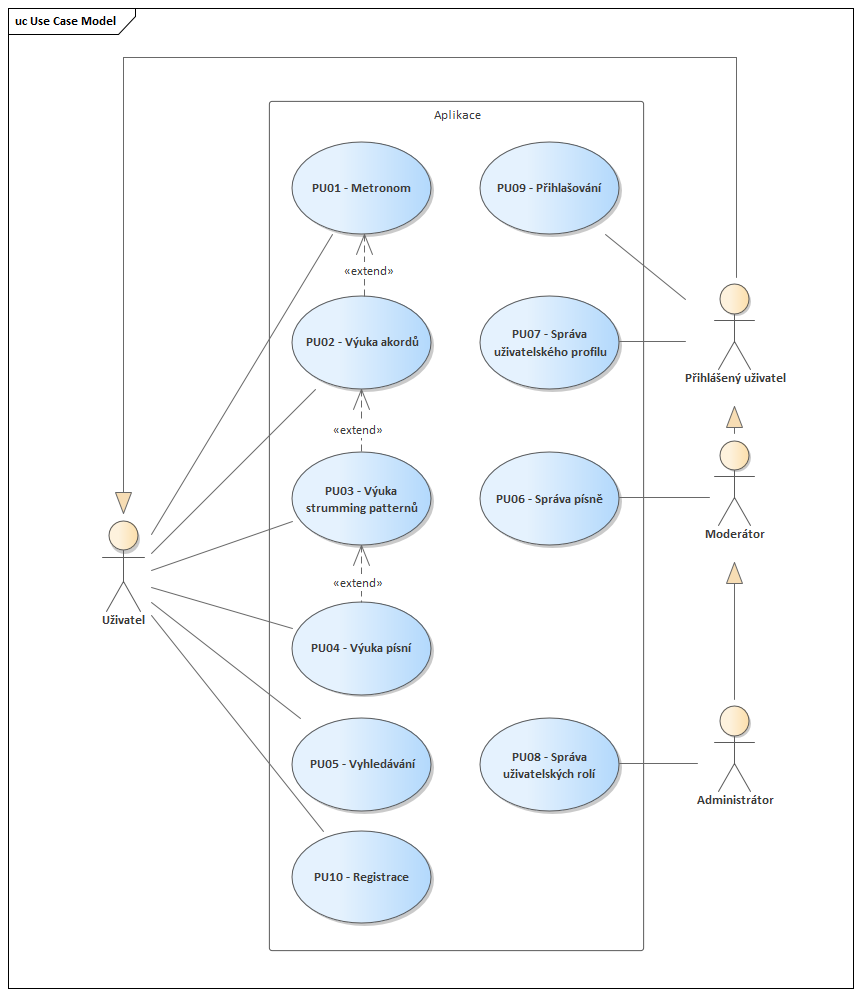
\includegraphics[width=0.9\textwidth]{assets/use_case_model.png}
    \caption{Diagram případu užití}
    \label{fig:use_case}
\end{figure}

\section{Návrh uživatelského rozhraní}
\label{sc:wireframes}
Návrh uživatelského rozhraní je důležitá součást vývoje software, protože to je ta část, kterou vidí uživatel. Sebelepší funkcionalita je aplikaci k~ničemu, když bude nepřehledná a příliš komplikovaná. Je několik možností, jak přistoupit k~takovému návrhu, dělené podle úrovně detailu, kterým se zabývají.

Nejvíce abstraktní, resp. nejméně se zabývající detaily je wireframe. Wireframe ukazuje část aplikace, její rozvržení a zabývá se pouze důležitými částmi. Další úrovní je mockup, který se na rozdíl od wireframu věnuje i méně podstatným částem aplikace a detailům jako jsou třeba barevná schémata či typografie. Poslední, nejpokročilejší a zároveň nejkomplikovanější možností je prototyp. Prototyp rozšiřuje mockup o~interakce, popř. animace. Umožňuje simulovat interakce mezi částmi aplikace a reprezentuje podobu konečného produktu. Rozdíl mezi prototypem a konečným produktem je, že prototyp má většinou nasimulovaná data, která by aplikace jinak získávala z~backendu. Prototypy jsou většinou vytvářeny před vývojem samotné aplikace pro zjištění, zdali má vůbec smysl takovou aplikaci vytvářet. Pokud má vývojář či tým zadaný požadavek na nějakou aplikaci, nemá smysl ztrácet čas s~prototypem, jelikož aplikaci musí dodat.

Práce uvažuje o~návrhu uživatelského rozhraní jako o~wireframu, jelikož v~kontextu této práce nemá smysl dělat prototyp. Co se týče výběru wireframu oproti mockupu, pak to je čistě subjektivní. V~praxi u~větších firem vyvíjející jednu z~mnoha aplikací je upřednostňován wireframe, jelikož detaily jako barevné schéma, či typografie se odvíjí od dalších aplikací a firemních politik. Wireframy jsou v~rozlišení $1920 \times 1080$ pixelů, tedy FullHD a byly vytvořeny v~nástroji \emph{figma.com}~\cite{figmainc_2019_figma}, který umožňuje vytváření wireframů, mockupů i prototypů.

\subsection{Stránka s~písní}
\label{ss:wireframe_song}
Nejdůležitější stránka celé aplikace. Jedná se o~komponentu z~\hyperref[uc04]{PU04}, tedy výuka písní a obsahuje komponenty~\hyperref[uc01]{Metronom},~\hyperref[uc02]{Akordy} a~\hyperref[uc03]{Strumming pattern}. Stránka obsahuje hlavní panel s~možností vyhledávání a tlačítka pro registraci a přihlášení. V~hlavní části je nejprve název písně, pak název autora a následně text a akordy písně. Zmíněné komponenty jsou po pravé straně, jelikož kdyby byly pozicovány nalevo, tak by se uživateli mohl číst špatně text, který by byl zarovnán vedle komponent. Celý obsah je na velké obrazovce odsazen na střed, tak aby se uživatel mohl soustředit pouze na část obrazovky.

\begin{figure}
    \centering
    \begin{subfigure}{\textwidth}
        \centering
        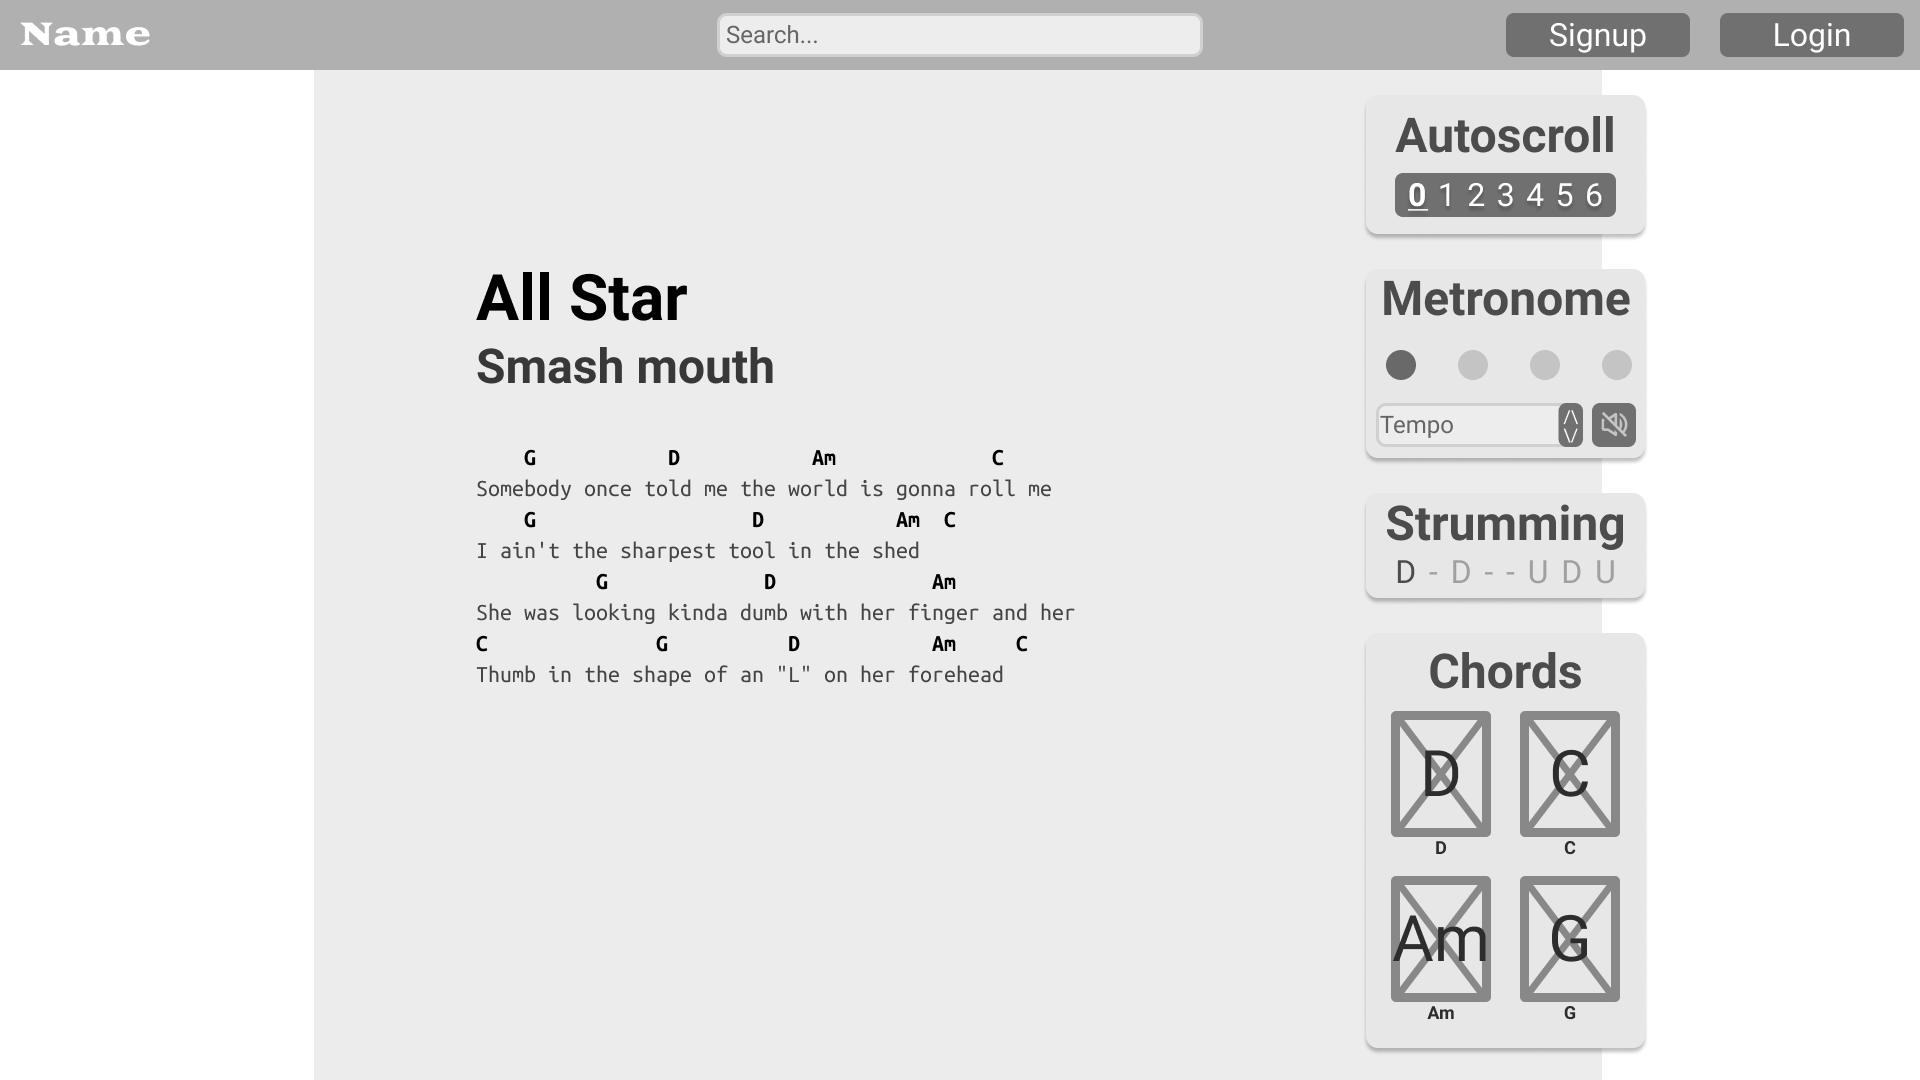
\includegraphics[width=\textwidth]{assets/song_page.png}
        \caption{Stránka s~písní}
        \label{fig:song_page}
    \end{subfigure}
    \par\bigskip
    \begin{subfigure}{.49\textwidth}
        \centering
        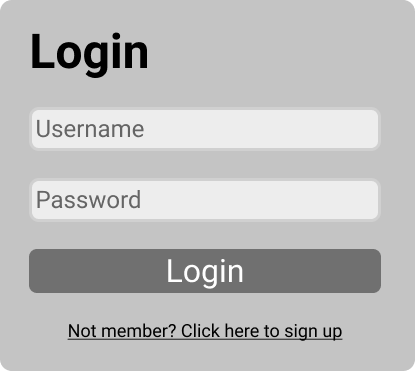
\includegraphics[width=.7\textwidth]{assets/login.png}
        \caption{Přilašovací okno}
        \label{fig:login_modal}
    \end{subfigure}
    \begin{subfigure}{.49\textwidth}
        \centering
        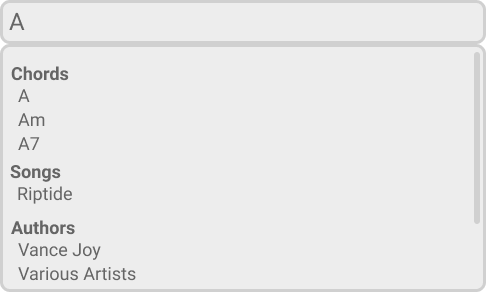
\includegraphics[width=.9\textwidth]{assets/search.png}
        \caption{Vyhledávací našeptávač}
        \label{fig:search}
    \end{subfigure}
    \caption{Wireframy}
    \label{fig:wireframes}
\end{figure}

% \begin{figure}
%     \begin{subfigure}{\textwidth}
%         \centering
%         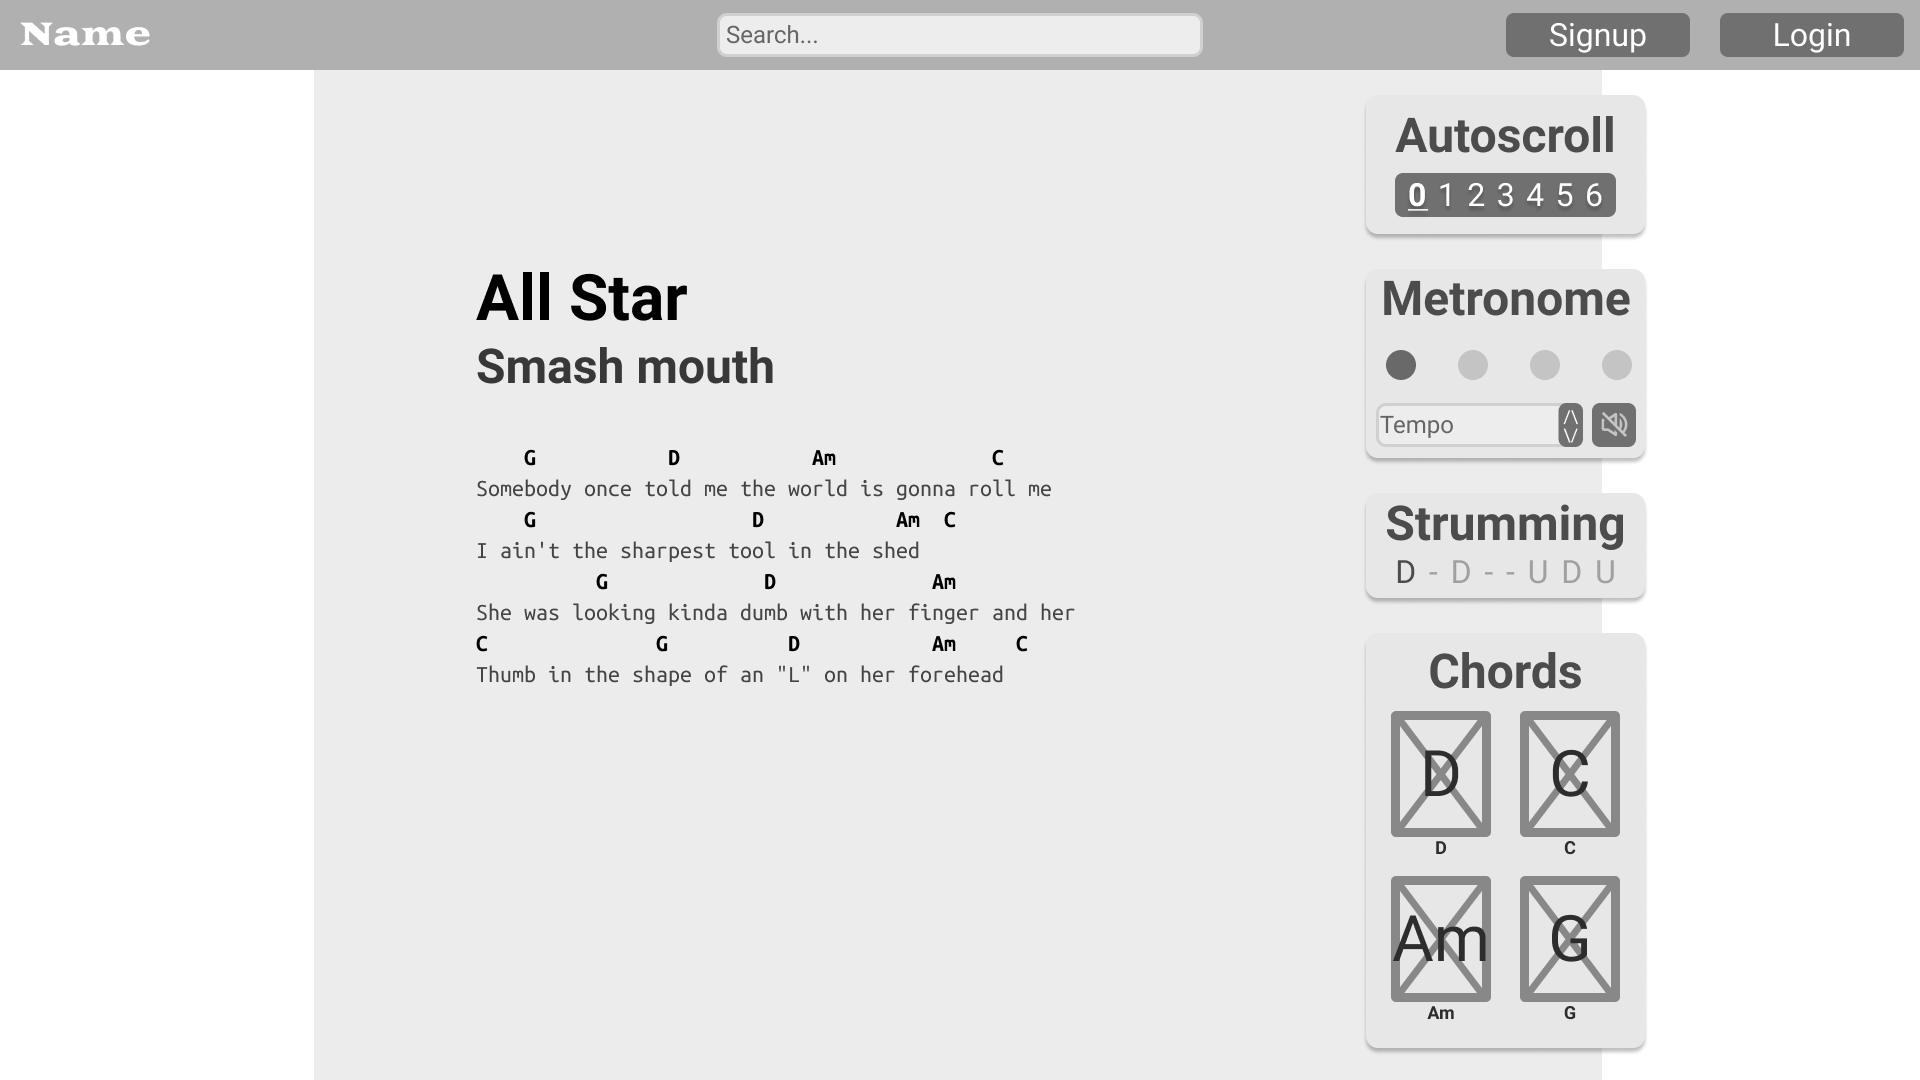
\includegraphics[width=\textwidth]{assets/song_page.png}
% \caption{Stránka s~písní}
% \label{fig:song_page}
%     \end{subfigure}

%     \medskip
%     \begin{subfigure}{.3\textwidth}
%         \centering
%         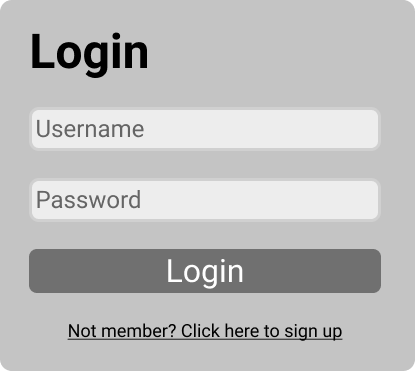
\includegraphics[width=.95\textwidth]{assets/login.png}
% \caption{Přilašovací okno}
% \label{fig:login_modal}
%     \end{subfigure}

%     \begin{subfigure}{.3\textwidth}
%         \centering
%         \includegraphics[width=.95\textwidth]{assets/signup.png}
%         \caption{Registrační okno}
%         \label{fig:signup_modal}
%     \end{subfigure}

%     \begin{subfigure}{.3\textwidth}
%         \centering
%         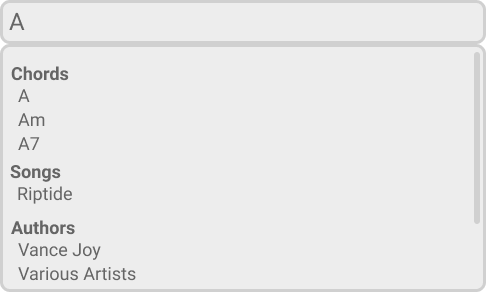
\includegraphics[width=.95\textwidth]{assets/search.png}
% \caption{Vyhledávací našeptávač}
% \label{fig:search}
%     \end{subfigure}


%     \caption{Wireframy}
%     \label{fig:wireframes}
% \end{figure}
